
\documentclass{beamer}

\usetheme{Blackboard}

\usepackage{mathpazo}

%\usepackage[latin1]{inputenc}
\usepackage[utf8x]{inputenc}
\usepackage[portuguese]{babel}
\usepackage[T1]{fontenc}

\usepackage{subfigure}

%%%%%%%%%%%%%%%%%%%%%%%%%%%%%%%%%%%%%%%%%%%%%%%%%%
%packages para usar letras gregas em negrito
\usepackage{bm} %opcao 2
%$\hat{\bm{\varphi}}
%%%%%%%%%%%%%%%%%%%%%%%%%%%%%%%%%%%%%%%%%%%5

%esse comando serve para deixar as equacoes mais curvadas, como no texto em latex
\usefonttheme[onlymath]{serif}

\usepackage{graphicx} % Allows including images
\usepackage{booktabs} % Allows the use of \toprule, \midrule and \bottomrule in tables

\titlegraphic{\pgfimage[height=0.8cm]{figuras/ufglogohorizontal.pdf}}

% \title{\centering \textbf{ Giroscópio}:} % The short title appears at the bottom of every slide, the full title is only on the title page

% \author{Discente: Itália Vallerini Barbosa. Orientador: Paulo Freitas Gomes}

% \institute[UFG-Jatai]{Universidade Federal de Goiás \\ UAE de Ciências Exatas\\ Regional Jataí \\% Your institution for the title page
% \medskip
% \textit{italia.vallerini@gmail.com} % Your email address
% }
% \date{23 de Fevereiro de 2018} % Date, can be changed to a custom date

\title{{\Huge Giroscópio e precessão: o que são?}}
\subtitle{{\LARGE E para que servem?}}
\author{{\Large Paulo Freitas Gomes}}%\footnote{\texttt{kmaeda@users.sourceforge.jp}}}


\begin{document}
\setbeamertemplate{footline}[page number] 

\begin{frame}
  \maketitle
\end{frame}

%   \AtBeginSection[]{% Print an outline at the beginning of sections
%     \begin{frame}<beamer>
%       \frametitle{Seção \thesection}
%       \tableofcontents[currentsection]
      

% \begin{frame}
% \titlepage % Print the title page as the first slide
% \end{frame}

\begin{frame}
\frametitle{Sum\'ario} 
\tableofcontents % Throughout your presentation, if you choose to use \section{} and \subsection{} commands, these will automatically be printed on this slide as an overview of your presentation
\end{frame}
%--------------------------------------------------------------------------------
%	PRESENTATION SLIDES

%------------------------------------------------
\section{Precessão} 


\begin{frame}
\frametitle{O que é precessão?}
\begin{itemize}
\item Precessão é a rotação do eixo de rotação de um objeto em torno de um segundo eixo.
\item É criado pelo torque da força peso (em geral) sobre o centro de massa quando o objeto está já em rotação. 
\pause
\item Não é um fenômeno intuitivo.
\item Porém mostra o quão sensacional é a grandeza momento angular!
\end{itemize}
\end{frame}



\begin{frame}
\frametitle{Precessão da Terra}
\begin{itemize}
\item O eixo de rotação da Terra sofre precessão: ele rotaciona em torno de outro eixo com um período de 26 mil anos.
\item O torque causador é exercido pela atração gravitacional da Lua e Sol.
\pause
\item Ainda há o movimento de nutação: oscilação em torno do cone de precessão.
\item Nutação e precessão da Terra são devido ao torque exercido pela Lua, Sol e outros planetas e pelo fato da Terra não ser uma esfera.
\end{itemize}
\end{frame}

\begin{frame}
\frametitle{Precessão da Terra}
\begin{figure}
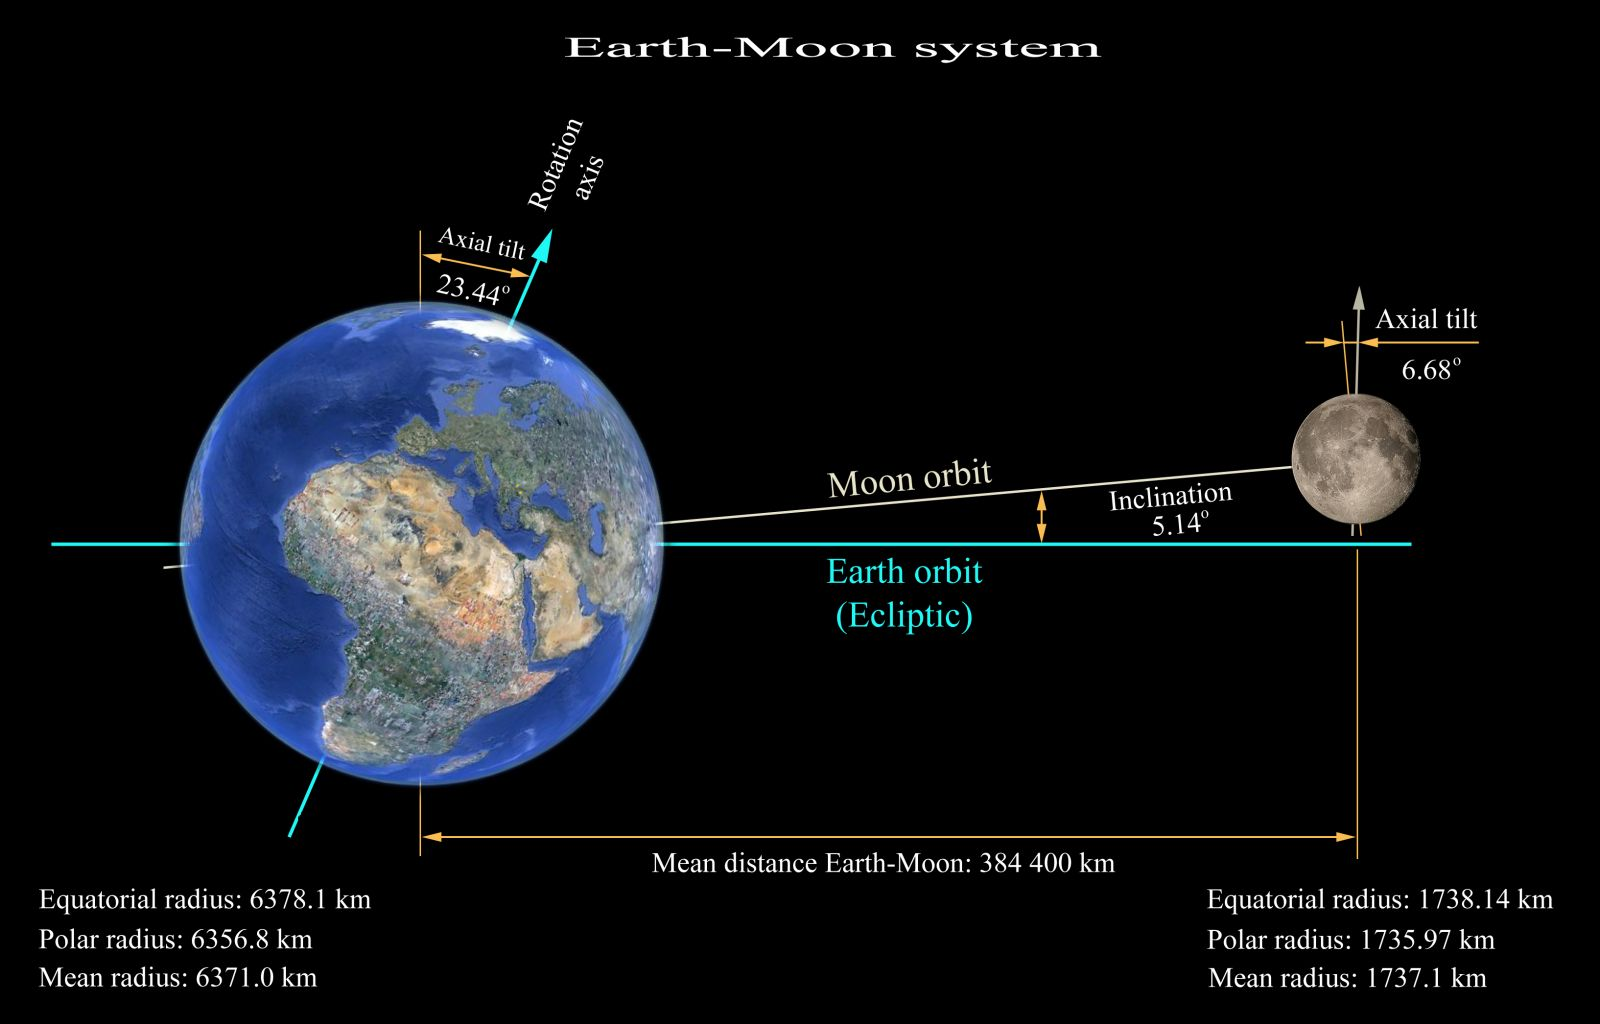
\includegraphics[width=4.0 in]{figuras/earth_moon_system.jpg}
%\caption{Fonte: \cite{Serway2014}.}
\end{figure}
\end{frame}


\begin{frame}
\frametitle{Precessão da Terra}
\begin{figure}
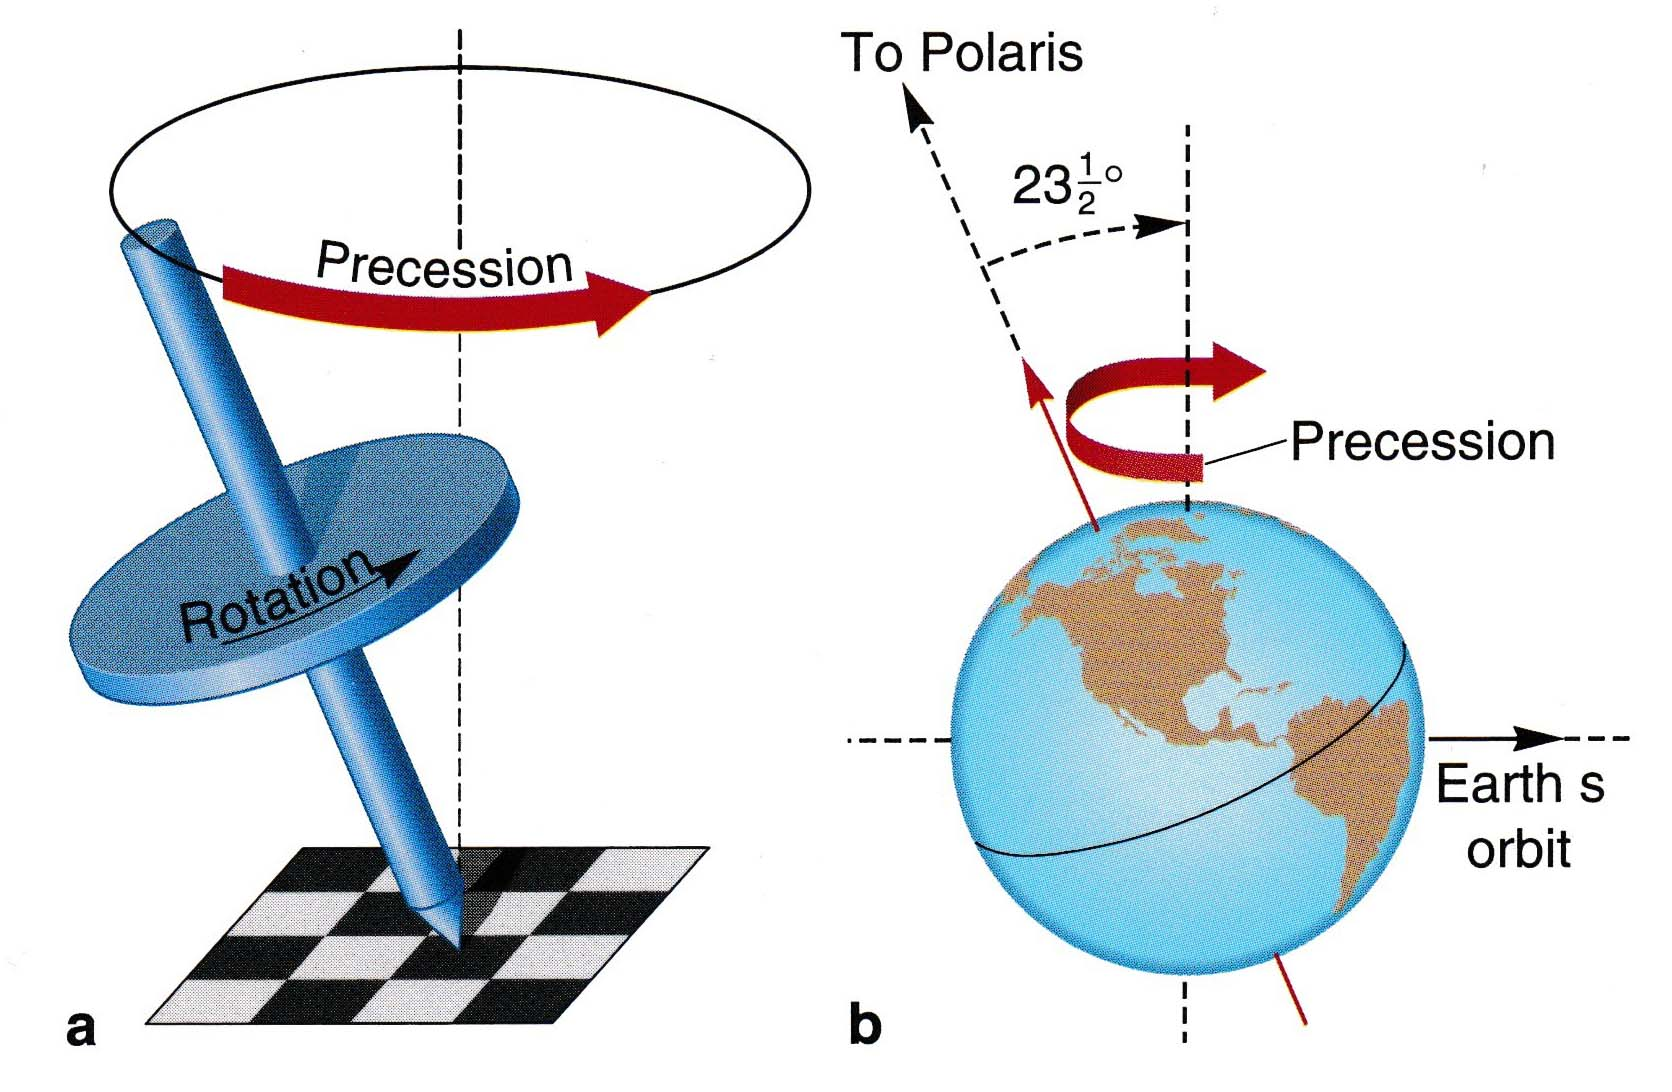
\includegraphics[width=3.9 in]{figuras/precession1a.jpg}
%\caption{Fonte: \cite{Serway2014}.}
\end{figure}
\end{frame}

\begin{frame}
\frametitle{Precessão da Terra}
\begin{figure}
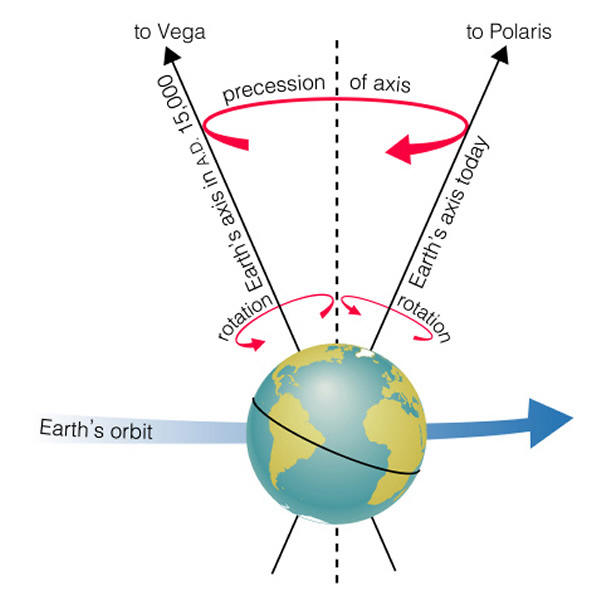
\includegraphics[width=2.2 in]{figuras/earthprecess.jpg}
%\caption{Fonte: \cite{Serway2014}.}
\end{figure}
\end{frame}






\begin{frame}
\frametitle{Precessão da Terra}
\begin{figure}
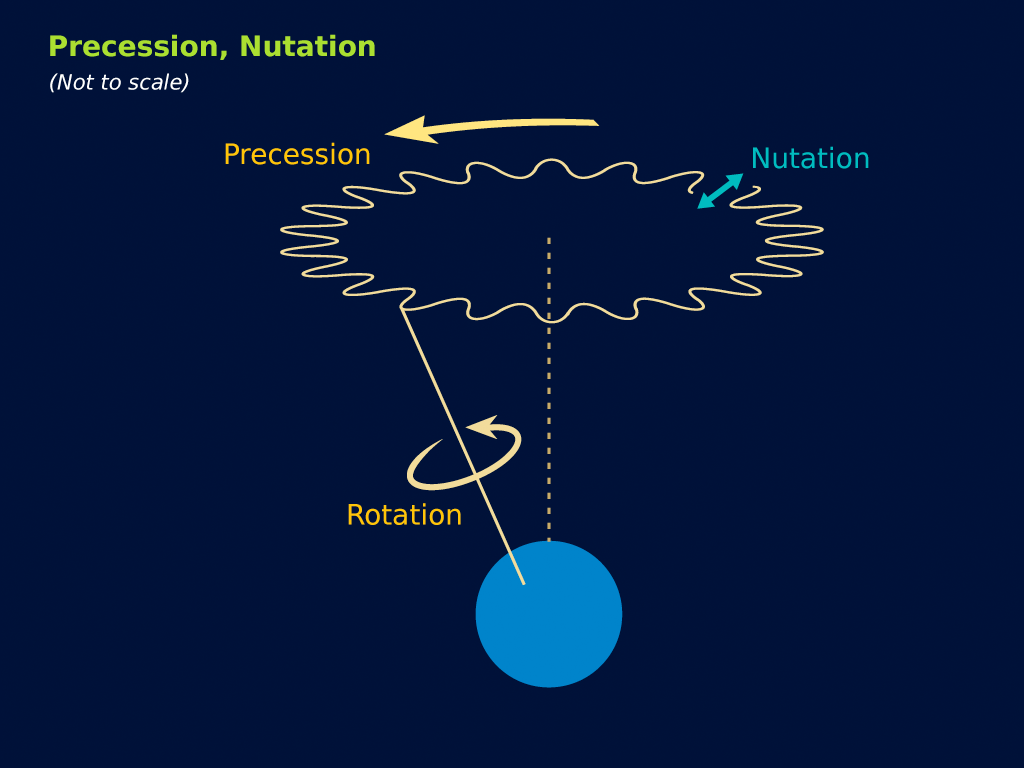
\includegraphics[width=3.7 in]{figuras/Precession_Nutation.png}
%\caption{Fonte: \cite{Serway2014}.}
\end{figure}
\end{frame}


\section{Giroscópio}


\begin{frame}
\frametitle{O que é giroscópio?}
\begin{itemize}
\item Giroscópio é um dispositivo contendo um rotor que rotaciona e outra parte externa que a sustenta. 
\item Independente de como a parte externa é suspensa a parte interna pode rotacionar livremente.
\item O atrito do suporte pode impedir uma rotação continuada do rotor.
\item Uma das aplicações do giroscópio é a observação da precessão.
\item Dentre as várias aplicações, o giroscópio é utilizado também para se observar a precessão.
\end{itemize}
\end{frame}


\begin{frame}
\begin{figure}
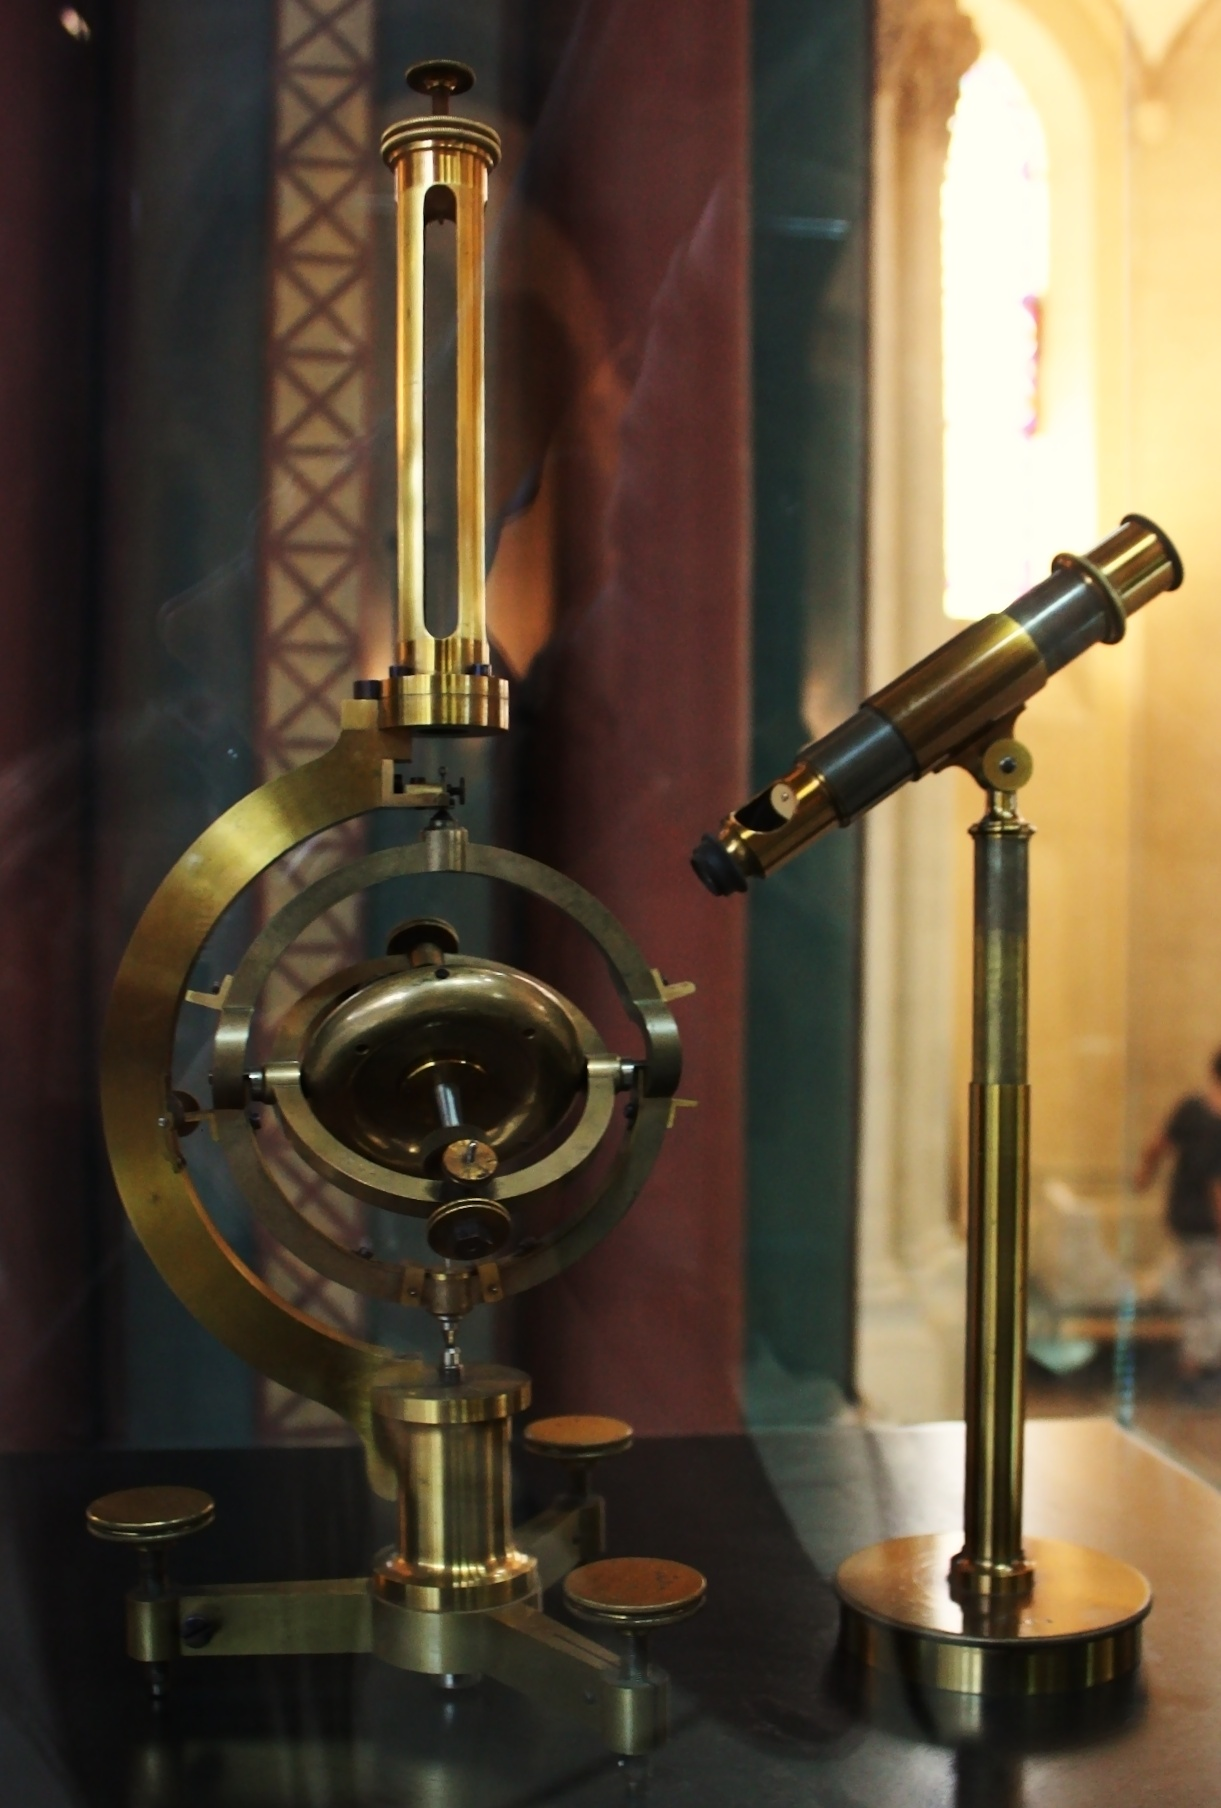
\includegraphics[width=2.0 in]{figuras/giroscopio_foucault.jpg}
\end{figure}
Giroscópio feito em 1852 por Léon Foucault.
\end{frame}

\begin{frame}
\begin{figure}
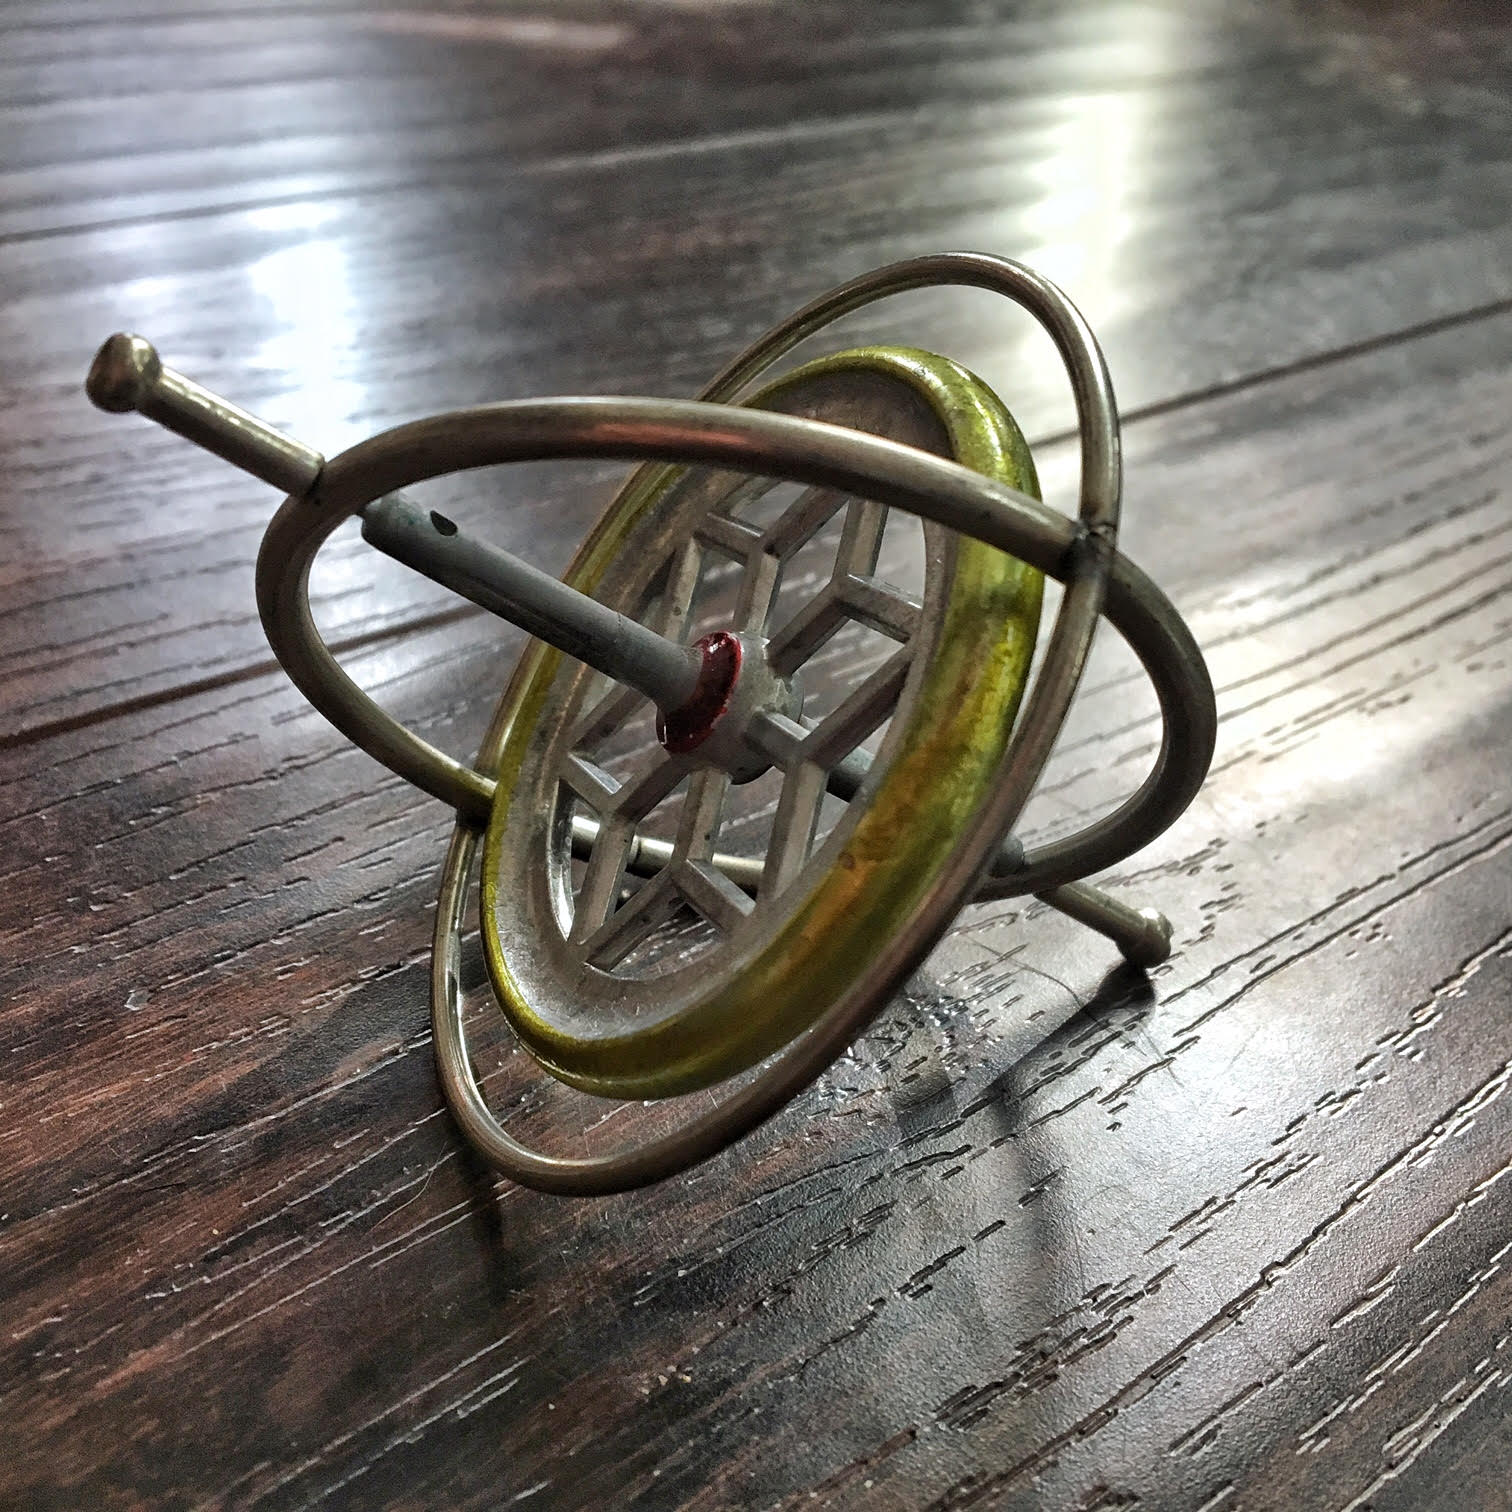
\includegraphics[width=3.0 in]{figuras/Gyroscope.jpg}
\end{figure}
Giroscópio de brinquedo da TEDCO Toys: criado em 1917.
\end{frame}

\begin{frame}
\begin{figure}
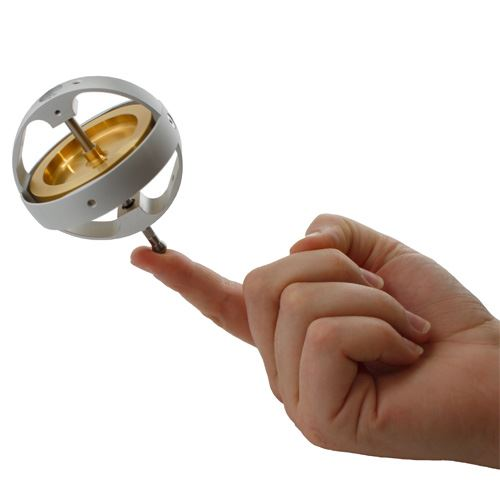
\includegraphics[width=3.0 in]{figuras/gyro3.jpg}
\end{figure}
\end{frame}

\begin{frame}
\begin{figure}
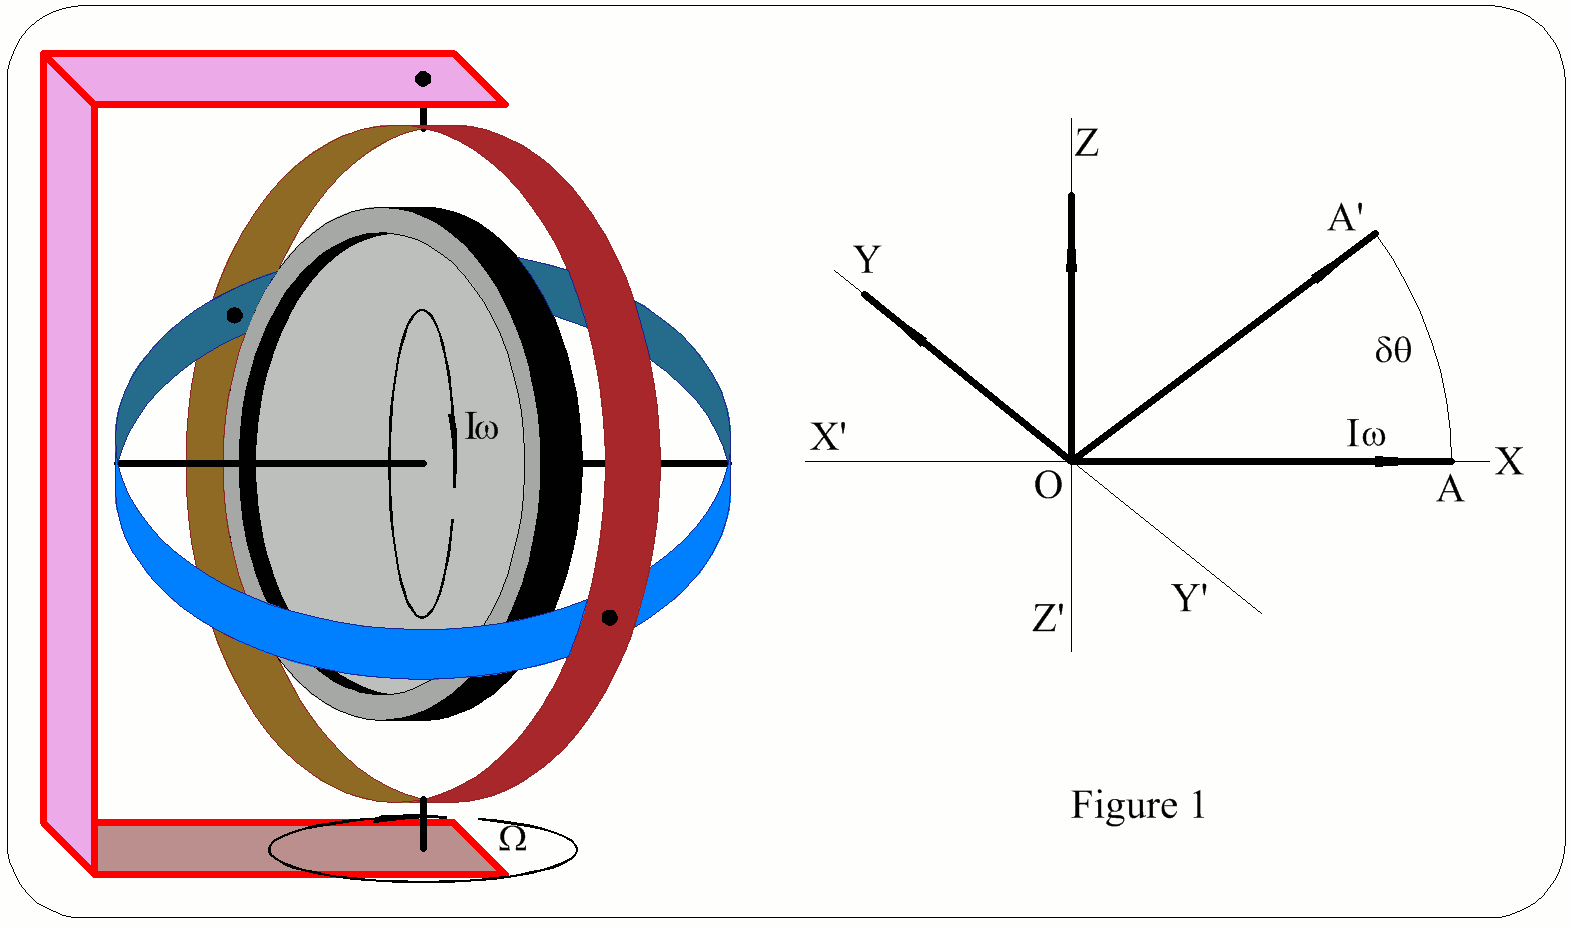
\includegraphics[width=4.2 in]{figuras/G1a.png}
\end{figure}
\end{frame}

\begin{frame}
\begin{figure}
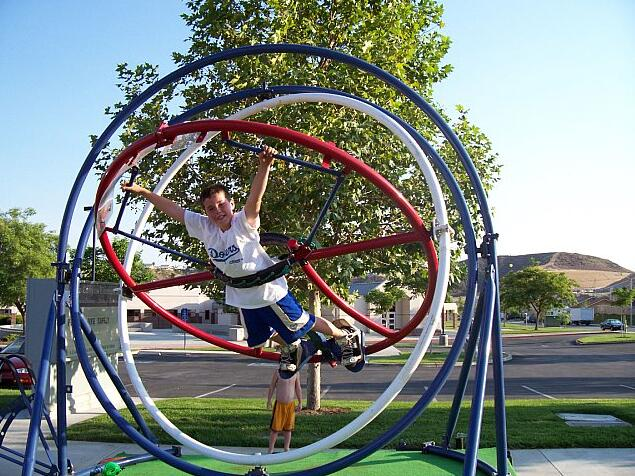
\includegraphics[width=3.9 in]{figuras/Human-Gyroscope.jpg}
\end{figure}
\end{frame}



\section{Modelo Teórico}

\begin{frame}
\frametitle{Definições}
%\framesubtitle{Definições}
\begin{itemize}
\item Grandezas vetoriais em negrito: {\color{red}$a=$} escalar e {\color{red}$\textbf{a}=$} vetor.
\item Momento Angular: {\color{red}$\textbf{L} = \textbf{r} \times \textbf{p} = m\textbf{r} \times \textbf{v} $}.
\item Torque: {\color{red}$\bm{\tau} = \textbf{r} \times \textbf{F}$}.
\item Torque da força peso: {\color{red}$\bm{\tau}_p = m\textbf{r} \times \textbf{g}$}.
\item Lei de Newton angular: {\color{red}$\bm{\tau} = \dfrac{d\textbf{L}}{dt}$}.
\end{itemize}
\end{frame}

\begin{frame}
%\frametitle{Introdu\c{c}\~ao}
\begin{figure}
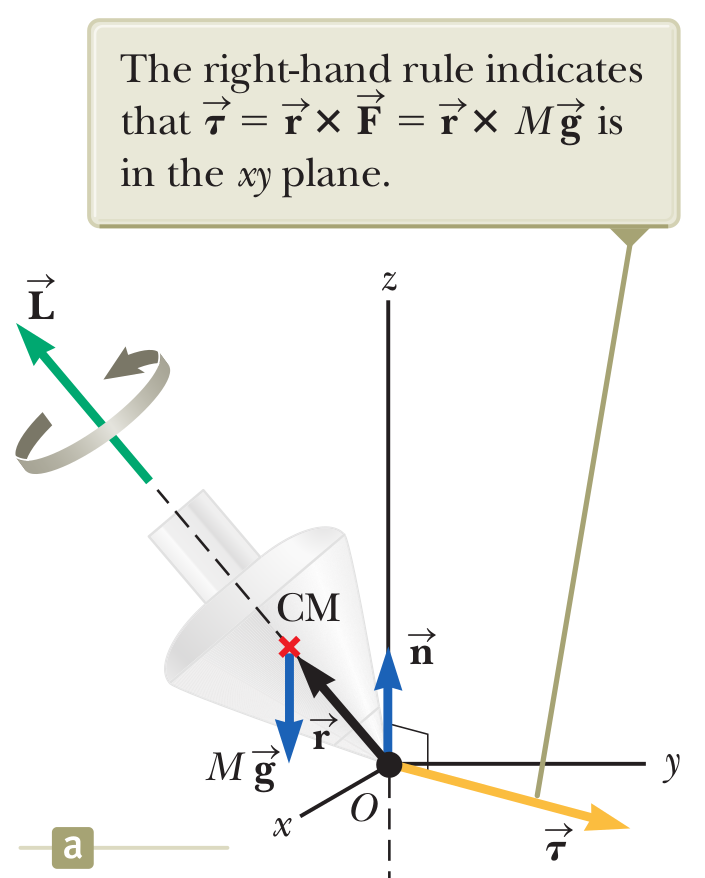
\includegraphics[width=2.2 in]{figuras/peao1.png}
\pause
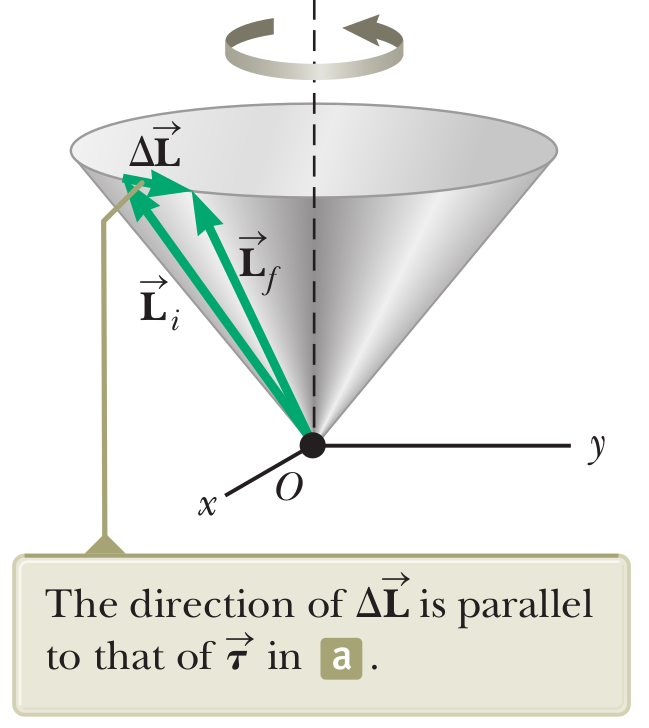
\includegraphics[width=2.2 in]{figuras/peao2.png}
\caption{Fonte: \cite{Serway2014}.}
\end{figure}
\end{frame}



\begin{frame}
\frametitle{Definições}
\begin{itemize}
\item O peão sofre duas forças: peso atuando no centro de massa e normal do chão no ponto de contato com o chão.
\item Seja {\color{red}$\textbf{r}$} no plano $yz$.
\item O peso faz um torque {\color{red}$\bm{\tau} = M\textbf{r} \times \textbf{g}=\hat{\textbf{i}}\tau$} paralelo ao eixo $x$.
\pause
\item Logo, da Lei de Newton: {\color{red}$d\textbf{L} = \bm{\tau}dt$}.
\item Isso faz o momento angular girar: {\color{red}$\textbf{L} = \textbf{L}_0 + \bm{\tau}dt$}.
\item Já que {\color{red}$\textbf{L}_0 \cdot \bm{\tau}=0$}: {\color{red}$\textbf{L}_0$} e {\color{red}$\bm{\tau}$} são perpendiculares.
\pause
\item Assim apenas a direção do momento angular {\color{red}$\textbf{L}$} é alterada.
\item O movimento de {\color{red}$\textbf{L}$} é chamado de precessão.
\end{itemize}
\end{frame}


\begin{frame}
%\frametitle{Introdu\c{c}\~ao}
\begin{figure}
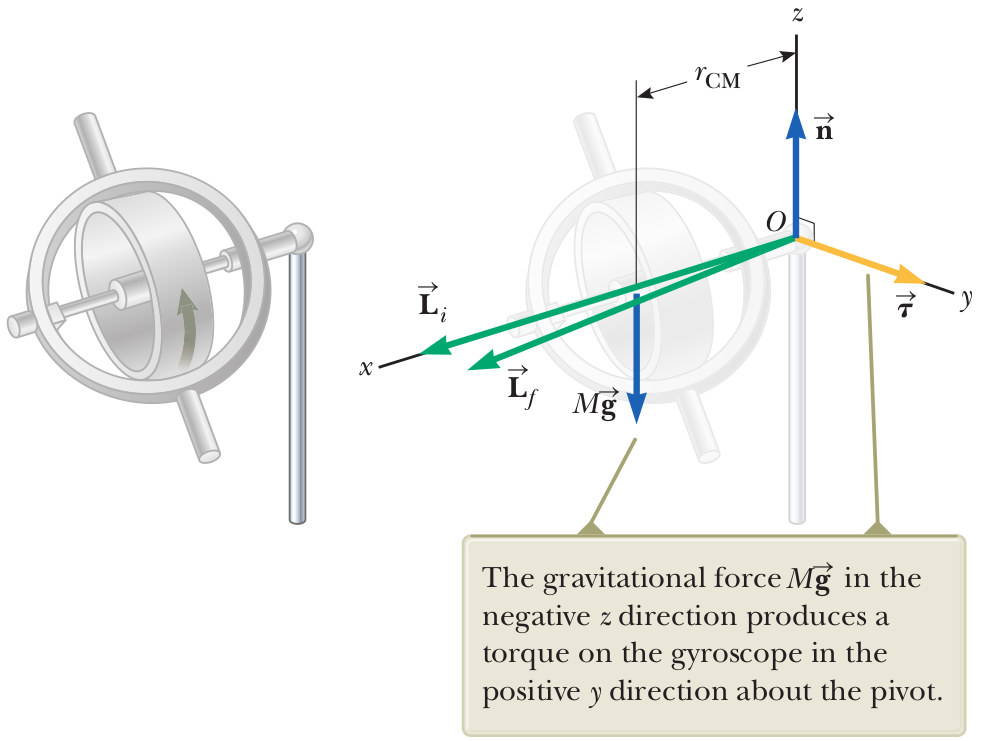
\includegraphics[width=3.6 in]{figuras/giroscopio1.png}
\caption{Fonte: \cite{Serway2014}.}
\end{figure}
\end{frame}


\begin{frame}
%\frametitle{Introdu\c{c}\~ao}
\begin{figure}
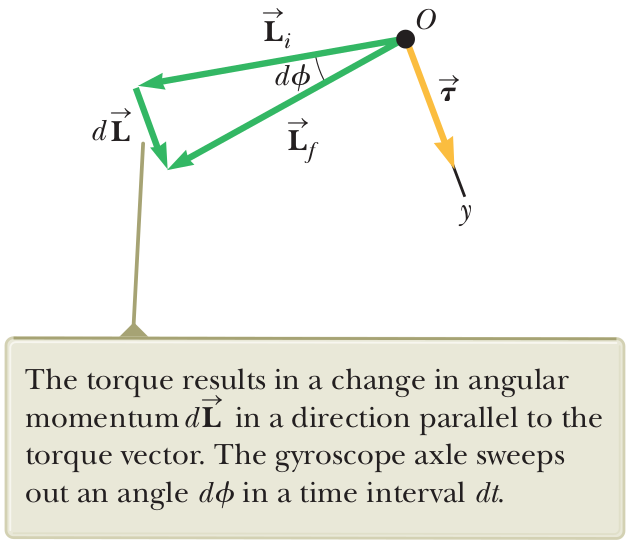
\includegraphics[width=3.4 in]{figuras/giroscopio2.png}
\caption{Fonte: \cite{Serway2014}.}
\end{figure}
\end{frame}


\begin{frame}
\frametitle{Velocidade angular de precessão}
\begin{itemize}
\item Do triângulo da figura anterior: {\color{red}$d\phi = \dfrac{dL}{L} = \dfrac{\tau dt}{L} = \dfrac{r F  }{I \omega}dt$}.
\item Logo a velocidade angular de precessão é:
{\color{red}\begin{equation}
\Omega = \dfrac{d\phi}{dt} = \dfrac{F r}{I \omega}, \nonumber
\end{equation}}
onde {\color{red}$F$} é a força que executa o torque.
\item Em geral é o peso {\color{red}$F=Mg$}.
\item Este resultado é valido quando {\color{red}$\Omega << \omega$}.
\end{itemize}
\end{frame}

%---------------------------------------------------



%-------------------------------------------------------
\section{Aplicações}
%-------------------------------------------------------


\begin{frame}
\frametitle{Aplicações}
\begin{itemize}
\item Giroscópios são dispositivos que mantem uma rotação independente da maneira com que são suportados.
\item Que aplicação isso teria?
\pause
\item Suponha que o giroscópio tenha seu rotor rotacionando. Quando o suporte é rotacionado, há então um movimento relativo entre ambos.
\item As aplicações residem ai: detecção desse movimento relativo!
\item Conectando o giroscópio em algo, pode-se saber quando esse algo rotaciona e então executar alguma função.
\end{itemize}
\end{frame}


\begin{frame}
\frametitle{Aplicações}
\begin{itemize}
\item Conectando o giroscópio em alguma estrutura, pode-se saber quando esse algo rotaciona e então executar alguma função.
\item Pode-se então determinar o ângulo de rotação (posição angular) dessa estrutura.
\item Isso significa então que podemos orientar essa estrutura da forma desejada.
\pause
\item A maior aplicação de giroscópios é estabilização!
\end{itemize}
\end{frame}

\begin{frame}
\frametitle{Estabilização}
\begin{itemize}
\item Câmeras, aeronaves e veículos podem ser mais estáveis com um sistema ativo que, dado a rotação do giroscópio, executa o movimento contrário para o veículo permanecer imóvel. 
\item Os instrumentos no helicóptero que indicam sua orientação são baseados em giroscópios.
\end{itemize}
\end{frame}

\begin{frame}
\frametitle{Smartphones e tablets}
\begin{itemize}
\item Giroscópios "eletrônicos" (MEMS-based) são amplamente utilizados em celulares e tables.
\item Combinado com acelerômetro e magnetômetro, obtém-se resultados precisos para a localização, posição e movimento do aparelho.
\item Aplicativos diversos exploram essa capacidade.
\end{itemize}
\end{frame}




\begin{frame}
%\frametitle{Introdu\c{c}\~ao}
\begin{figure}
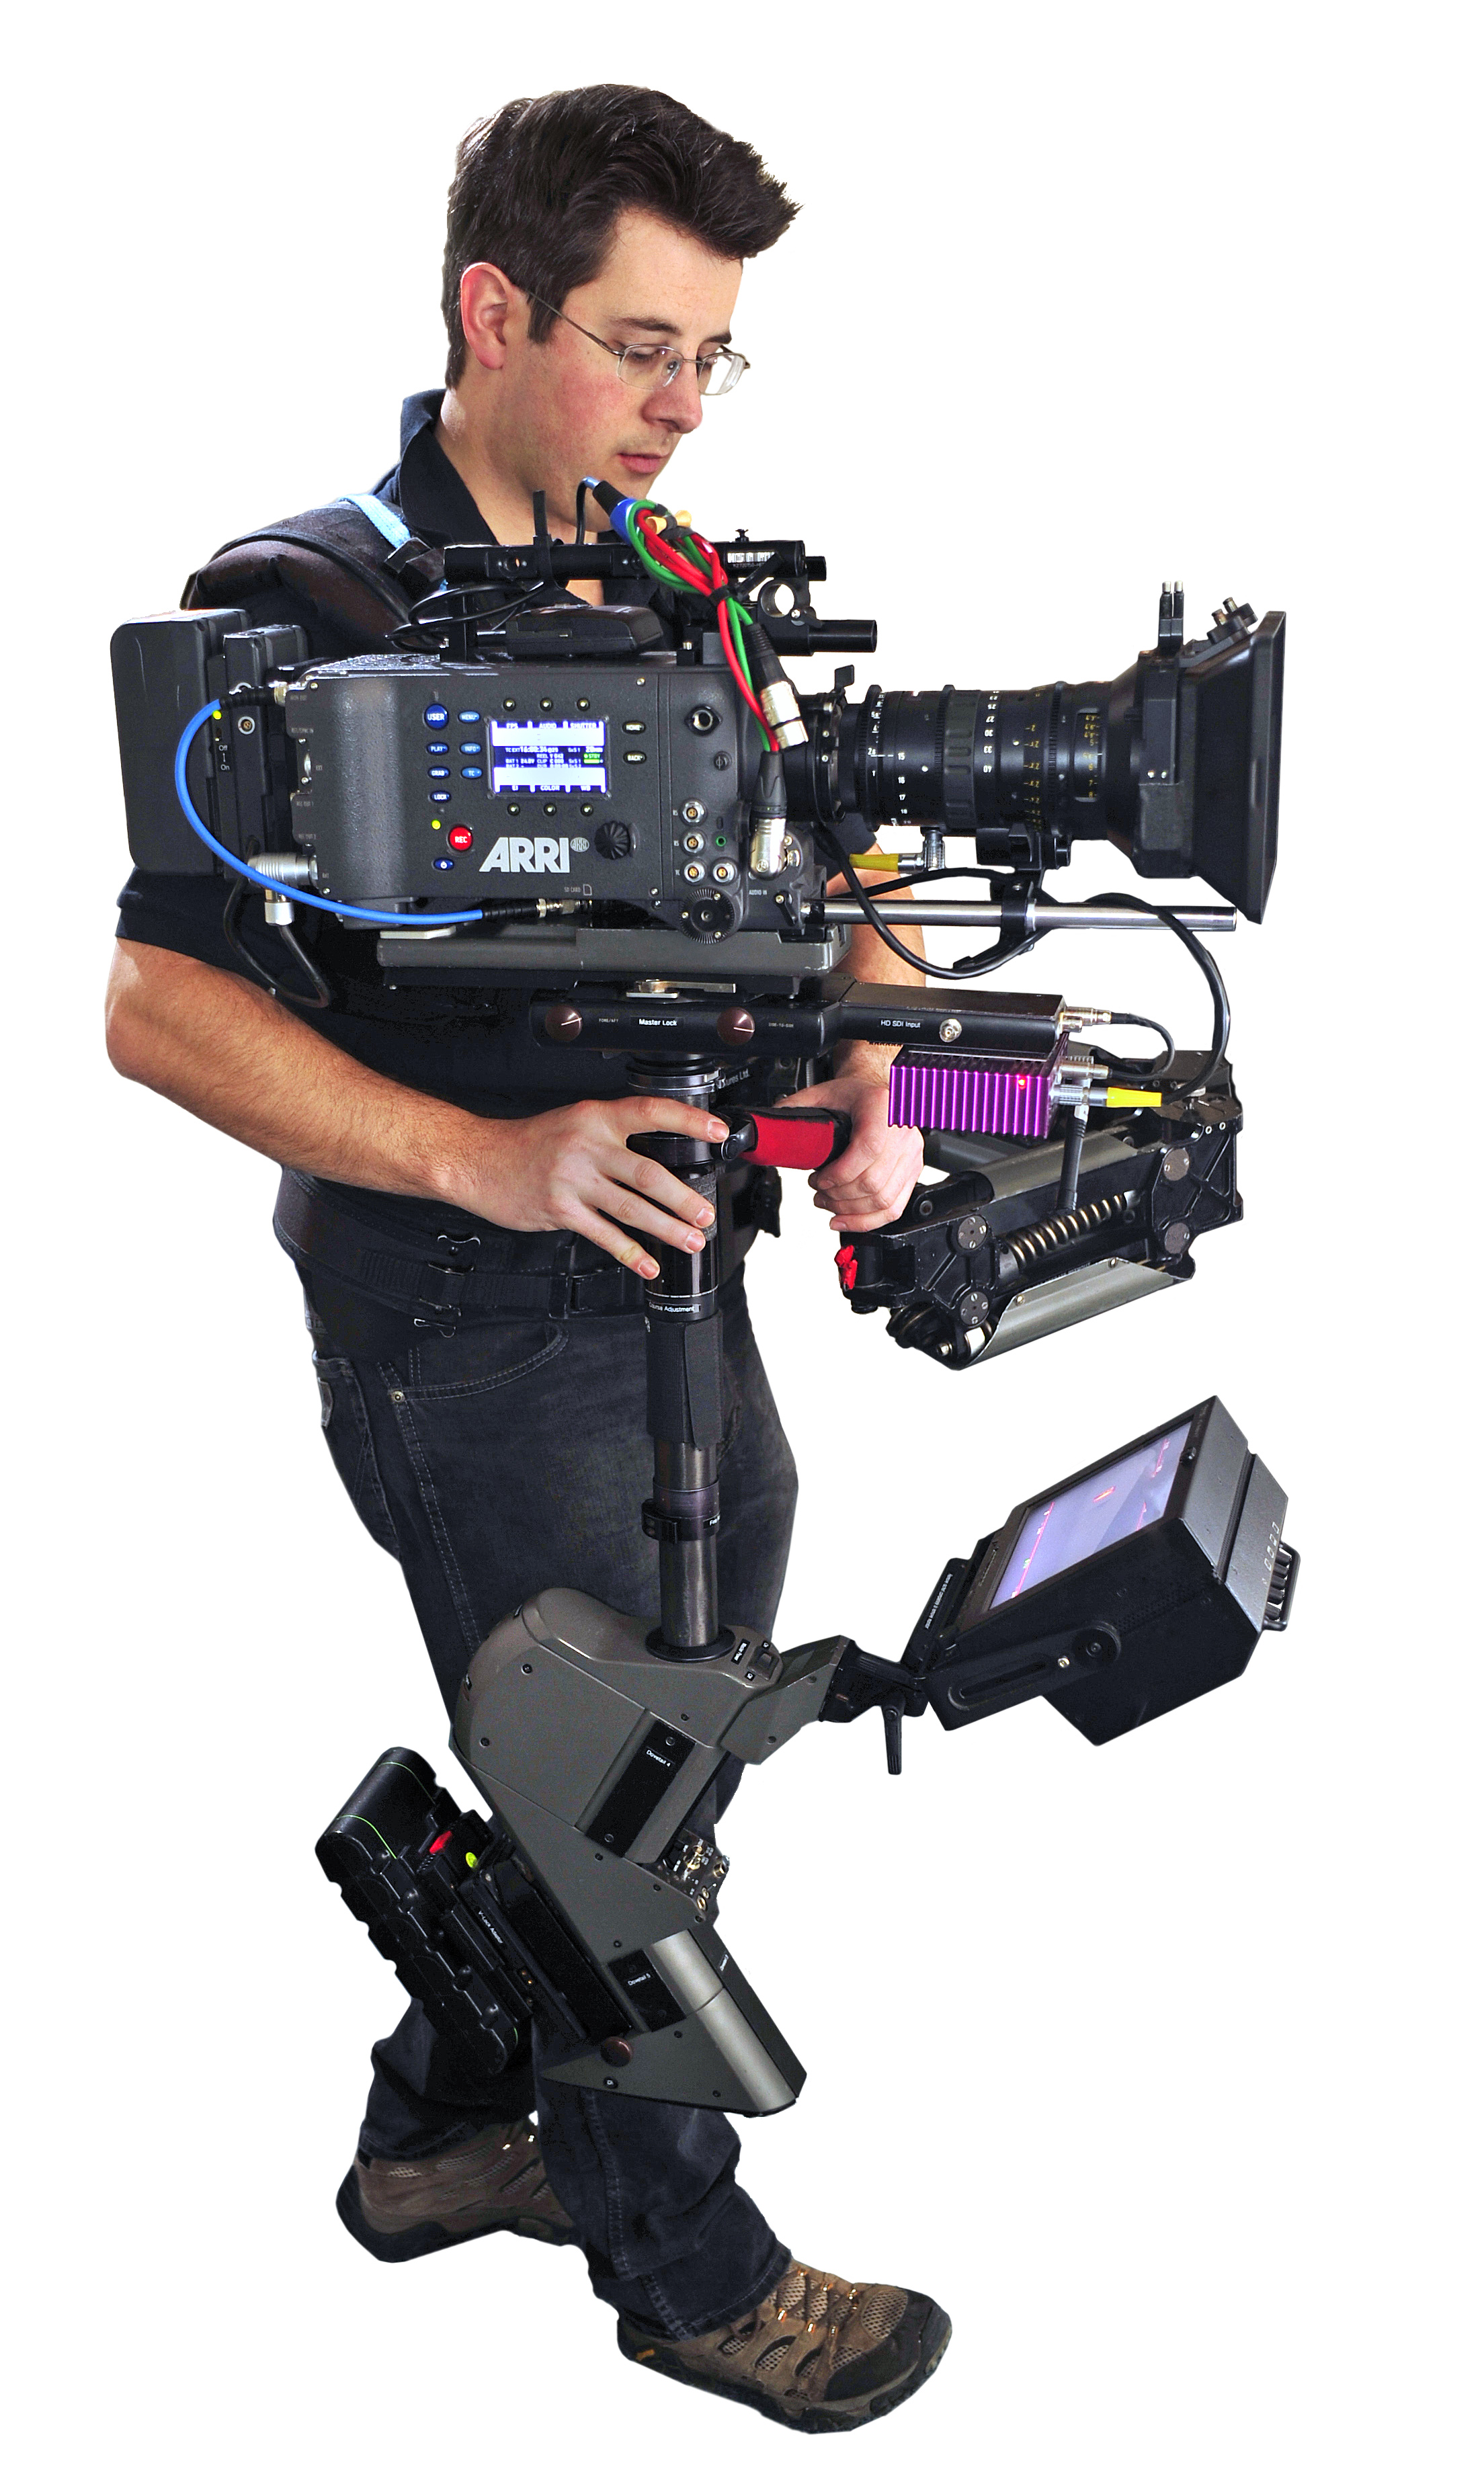
\includegraphics[width=2.0 in]{figuras/camera.jpg}
%\caption{Ilustração dos processos possíveis na interação entre radiação e matéria.}
\end{figure}
\end{frame}


\begin{frame}
\begin{figure}
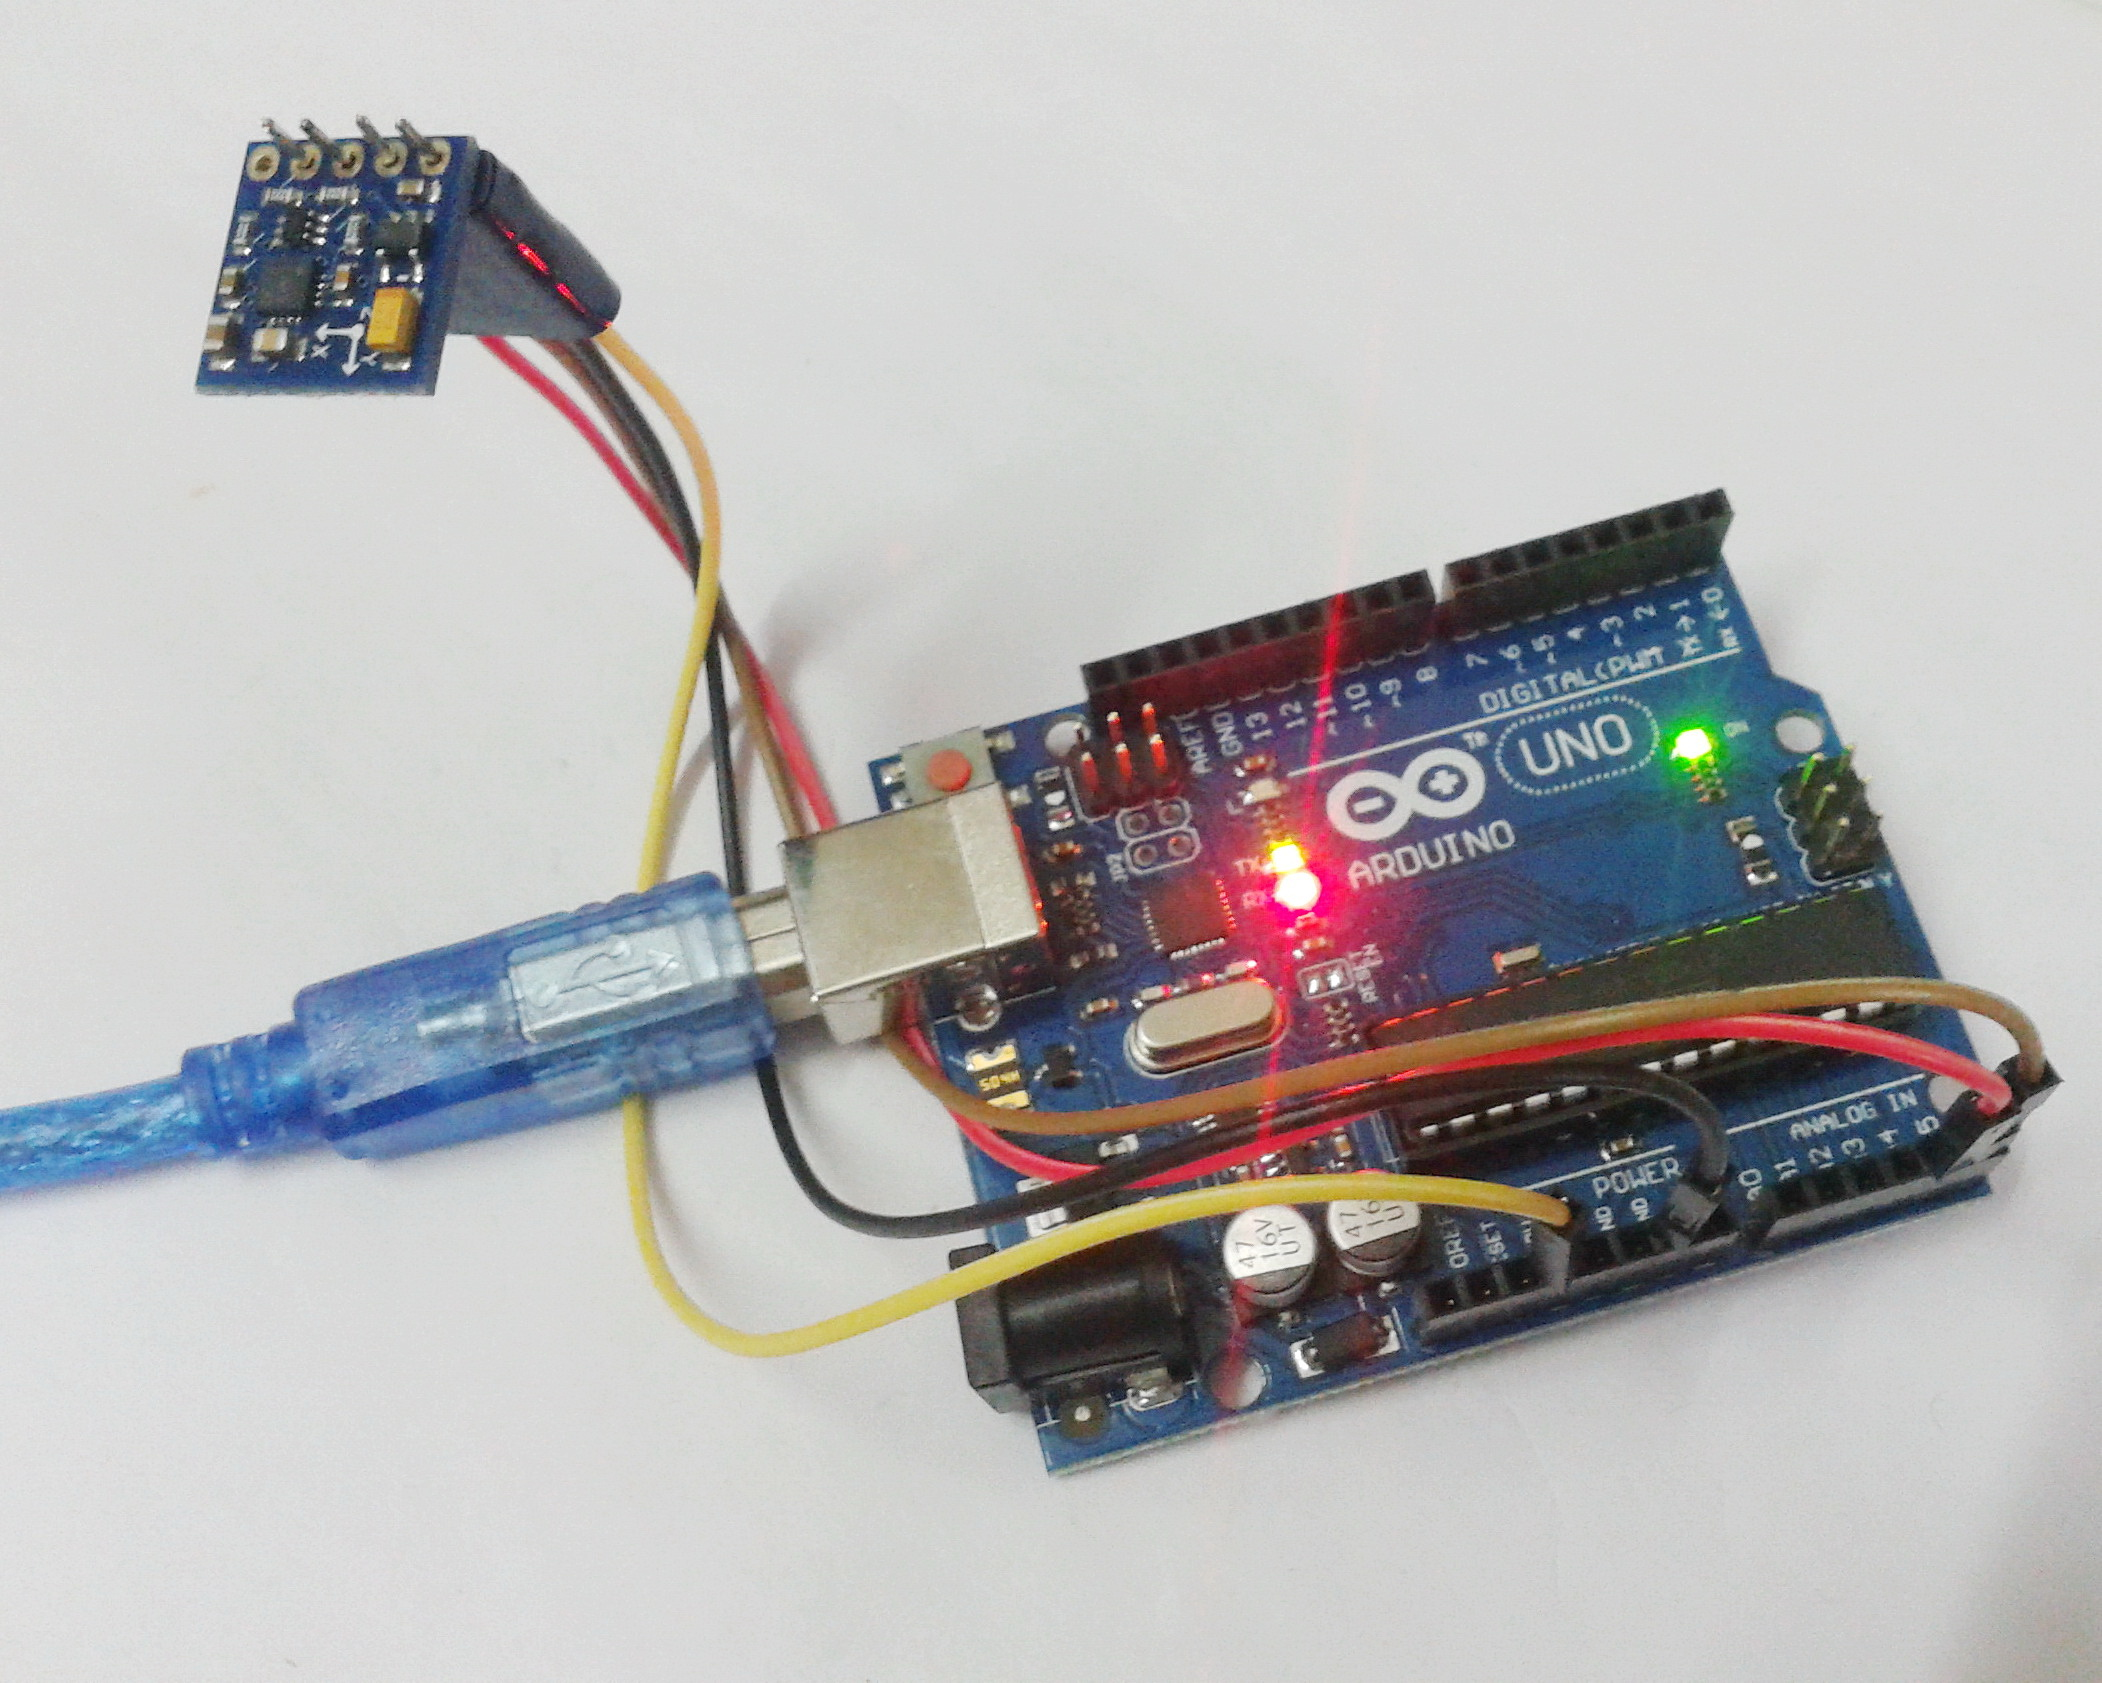
\includegraphics[width=3.5 in]{figuras/Arduino.jpg}
\end{figure}
Micro controlador Arduino acoplado com um sensor giroscópio.
\end{frame}


\begin{frame}
\begin{figure}
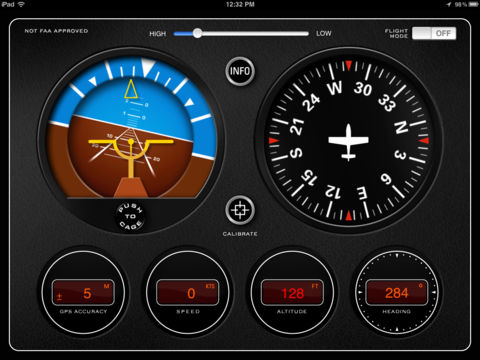
\includegraphics[width=3.5 in]{figuras/aviao.jpg}
\end{figure}
Micro controlador Arduino acoplado com um sensor giroscópio.
\end{frame}



\begin{frame}
\begin{figure}
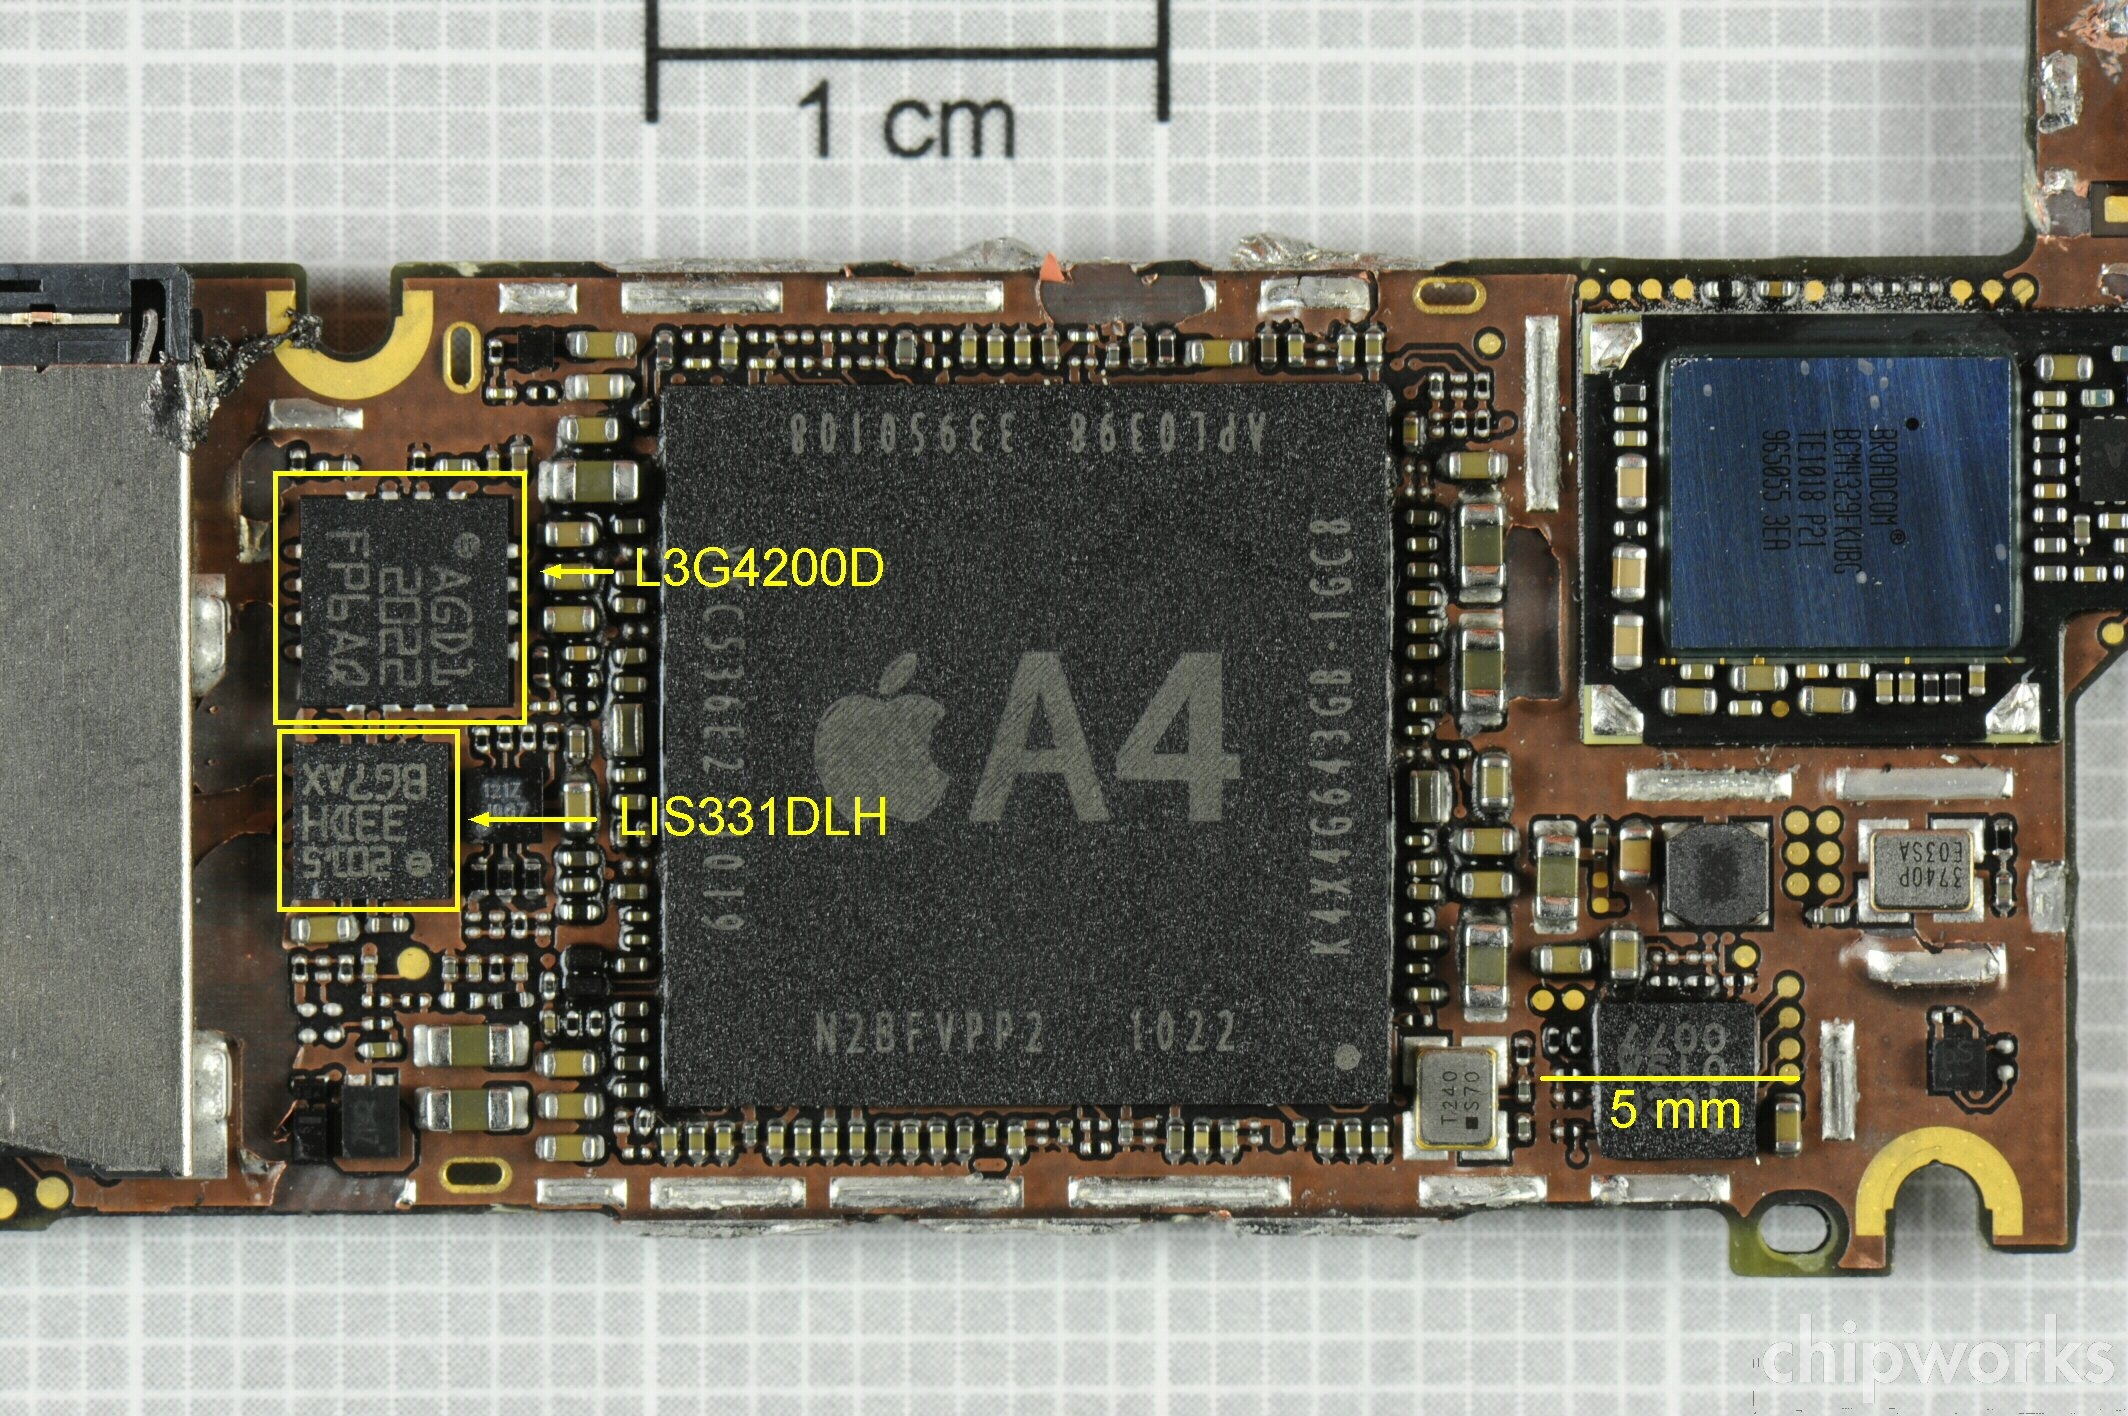
\includegraphics[width=3.7 in]{figuras/giroscopio_iphone.jpg}
\caption{O giroscopio é o L3G4200D.}
\end{figure}
\end{frame}







\begin{thebibliography}{9}

      \begin{frame}[label=bibliography]{Bibliography}
      %\framesubtitle{\TeX, \LaTeX, and Beamer}
      
\bibitem{Serway2014} R. A. Serway, J. W. Jewett, Jr, \textit{Physics: for Scientists and Engineers}, 9th edition Brooks/Cole Cengage Learning 2014.

    \end{frame}
    \end{thebibliography}

\begin{frame}
\Huge{\centerline{Obrigado!}}
\end{frame}

%----------------------------------------------------------------------------------------

\end{document}